\documentclass[handout]{beamer}

\usepackage[utf8]{inputenc}
\usepackage{tikz}
\usepackage{drawstack}
\usepackage{listings}
\usepackage{caption}

\usetikzlibrary{shapes.multipart,arrows}

% Setup
\title{Abstract Machine~\\for Modern Programming Languages}
\author[Altschuler, Færevaag]{Simon Altschuler (s123563) \and Markus Færevaag (s123692)}
\date{Software Technology Bachelor Thesis, Spring 2015}
\subject{Computer Science}

% Style
\usetheme{Berlin}
\usecolortheme{beaver}
\usefonttheme{structuresmallcapsserif}
\beamertemplatenavigationsymbolsempty{}
\setbeamertemplate{footline}[frame number]
\setbeamertemplate{itemize item}[circle]
\setbeamertemplate{itemize subitem}[triangle]
\setbeamertemplate{enumerate items}[default]
\definecolor{lered}{rgb}{0.58, 0.02, 0.03}
\setbeamercolor{itemize item}{fg=lered}
\setbeamercolor{itemize subitem}{fg=lered}

\newcommand{\n}[1]{\leavevmode\\~\texttt{\color{red}\tiny #1}}
% \newcommand{\n}[1]{}

\begin{document}

\frame{\titlepage}

\begin{frame}
  \frametitle{Motivation}
  \framesubtitle{Reasons for working on this project}

  Problem
  \begin{itemize}
  \item Available machines are unsuitable for modern paradigms
    \n{Not supporting dynamic and functional languages}
  \item Heavy focus on object-orientated and imperative languages
  \end{itemize}

  \pause{}

  \vspace{20pt}
  Learning
  \begin{itemize}
  \item Abstract machines are used everywhere
    \n{Browsers, mobile devices, desktop apps, embedded systems, similar to compilers/interpreters}
  \item Embody a broad spectrum of computer science topics
    \n{Compiler theory, lots of data structures, optimizations, low-level stuff}
  \end{itemize}

\end{frame}

\begin{frame}
  \frametitle{Contributions}
  \framesubtitle{Division of Responsibility}

  \begin{columns}[onlytextwidth, t]
    \begin{column}{0.33\textwidth}
      Shared
      \fontsize{9pt}{15}\selectfont
      \begin{itemize}
      \item Object model
      \item Stack
      \item Core architecture
      \item Testing
      \item Debugging facilities
      \end{itemize}
    \end{column}

    \pause{}

    \begin{column}{0.33\textwidth}
      Simon
      \fontsize{9pt}{15}\selectfont
      \begin{itemize}
      \item Instruction cycle
      \item Execution model
      \item ELF
      \end{itemize}
    \end{column}

    \pause{}

    \begin{column}{0.33\textwidth}
      Markus
      \fontsize{9pt}{15}\selectfont
      \begin{itemize}
      \item Type system
      \item Threads
      \item Information tables
      \end{itemize}
    \end{column}
  \end{columns}

  \pause{}

  \vspace{30pt}
  \centering
  We have both been involved in everything!

\end{frame}

\begin{frame}
  \frametitle{Agenda}
  \fontsize{11pt}{20}\selectfont
  \begin{enumerate}[<+->]
  \item Abstract machines 101
    \n{Simon}
  \item Existing systems
    \n{Markus}
  \item Matisse and the multi-paradigm approach
    \n{Simon}
  \item Implementation
    \n{Markus}
  \item Demo
    \n{Simon}
  \item Evaluation
    \n{Markus}
  \item Conclusions
    \n{Foo bar}
  \end{enumerate}
\end{frame}

\begin{frame}
  \frametitle{Abstract machines 101}

  Fundamentals

  \begin{itemize}[<+->]
  \item Virtual computer architecture
    \n{PROCESS not SYSTEM! Computer arch: organization of components}
  \item Hardware implemented in software
    \n{Shares properties of hardware like CPU/Memory mgmt/clock cycles}
  \item Executes low-level machine code
    \n{Machine code vary from very-low level to relatively high-level}
  \end{itemize}

\end{frame}

\begin{frame}
  \frametitle{Abstract machines 101}

  Advantages
  \begin{itemize}[<+->]
  \item Platform independence
    \n{Unified ISA, Just compile for new platforms}
  \item Expressive instruction set
    \n{Main reason, high-level constructs}
  \item Security
    \n{Sandboxed environment, cannot control access to system resources}
  \end{itemize}

  Disadvantages
  \begin{itemize}[<+->]
  \item Performance overhead
    \n{JIT = GG, but still some compilation overhead}
  \item Users must have the machine installed
    \n{Must be retrieved from somewhere, it must be available for the system}
  \end{itemize}

\end{frame}

\begin{frame}
  \frametitle{Abstract machines 101}

  How and where are they used
  \begin{itemize}[<+->]
  \item Web browsers
    \n{Java applet}
  \item Desktop applications
    \n{JVM, CIL, Parrot}
  \item Embedded devices
    \n{Hmm?}
  \item Virtualization
    \n{Hmm?}
  \end{itemize}

\end{frame}

\begin{frame}
  \frametitle{Existing systems}
  \framesubtitle{And their shortcomings}

  \begin{itemize}
  \item JVM and CLR
    \n{JVM (Java bytecode): Java and Scala, CLR (CIL): C\#, F\#, and more}
  \item Insufficient for modern paradigms
    \n{Object-Oriented by design, no flexibility\\
       Attempts to remedy: {\tt invokedynamic} and DLR
    }
  \item Interesting case: Parrot VM
    \n{Handled dynamic languages, but not static\\
       Does not solve our goals
     }
  \end{itemize}
\end{frame}

\begin{frame}
  \frametitle{Matisse}
  \framesubtitle{The Multi-Paradigm Approach}

  What distinguishes Matisse
  \begin{itemize}
  \item No paradigm assumptions
    \n{Attempted to be flexible enough to cover all}
  \item Achieved by exposing primitives
    \n{Building blocks for compilers, to use however they like. Scopes, fields, types, sub-routines}
  \item Opt-in features
    \n{Threading, scopes}
  \item Sub-routines are simple and sharable
    \n{They are just references and anon. could be generated easily}
  \item Flexible type system
    \n{AnyType is awesome for dynamic}
  \end{itemize}
\end{frame}

\begin{frame}
  \frametitle{Implementation}

  \n{Note why C: Speed and low-level flexibility}
  \n{Briefly each component}
  \n{Step through execution}

  \begin{figure}[H]
    \centering
    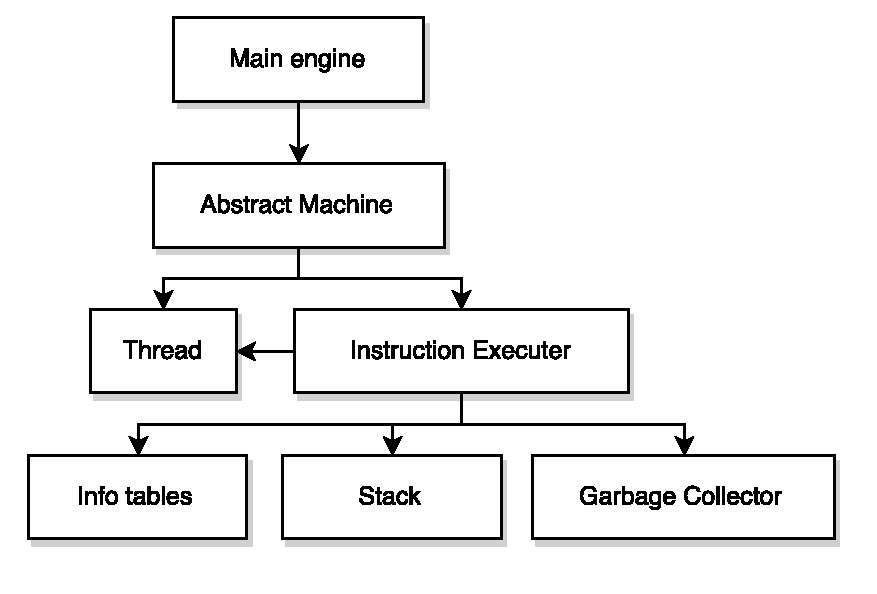
\includegraphics[scale=0.5]{../figures/arch.pdf}
  \end{figure}
\end{frame}

\begin{frame}
  \frametitle{Demo}
  \begin{itemize}
  \item Program 1
    \begin{itemize}
    \item Stack manipulation
    \item Sub-routines
    \item Arithmetic
    \end{itemize}

  \item Program 2
    \begin{itemize}
    \item Heap object
    \item Field manipulation
    \end{itemize}

  \item Complex program
  \end{itemize}
    % \item Demo program 1:
    %   \begin{itemize}
    %   \item push two ints
    %   \item add
    %   \item show stack
    %   \item make one int a float
    %   \item type error!
    %   \item box
    %   \item make sub-routine that takes the boxed int and adds one (and returns nothing)
    %   \item unbox the reference
    %   \item use `iprint' to print the result (strtab 4 is iprint)
    %   \end{itemize}

    % \item Demo program 2:
    %   \begin{itemize}
    %   \item new heap object (new, `person')
    %   \item push field `age' (should be 0)
    %   \item push an int
    %   \item pop to field `age'
    %   \end{itemize}

    % \item Show the fibo program as an example of a more complex thing
\end{frame}

\begin{frame}
  \frametitle{Performance Evaluation}
  \framesubtitle{Running time}

  \n{JIT with Mono}

  \begin{figure}
    \centering
    \begin{minipage}{.5\textwidth}
      \centering
          \scalebox{0.36}[0.3]{% Created by tikzDevice version 0.8.1 on 2015-06-27 20:39:43
% !TEX encoding = UTF-8 Unicode
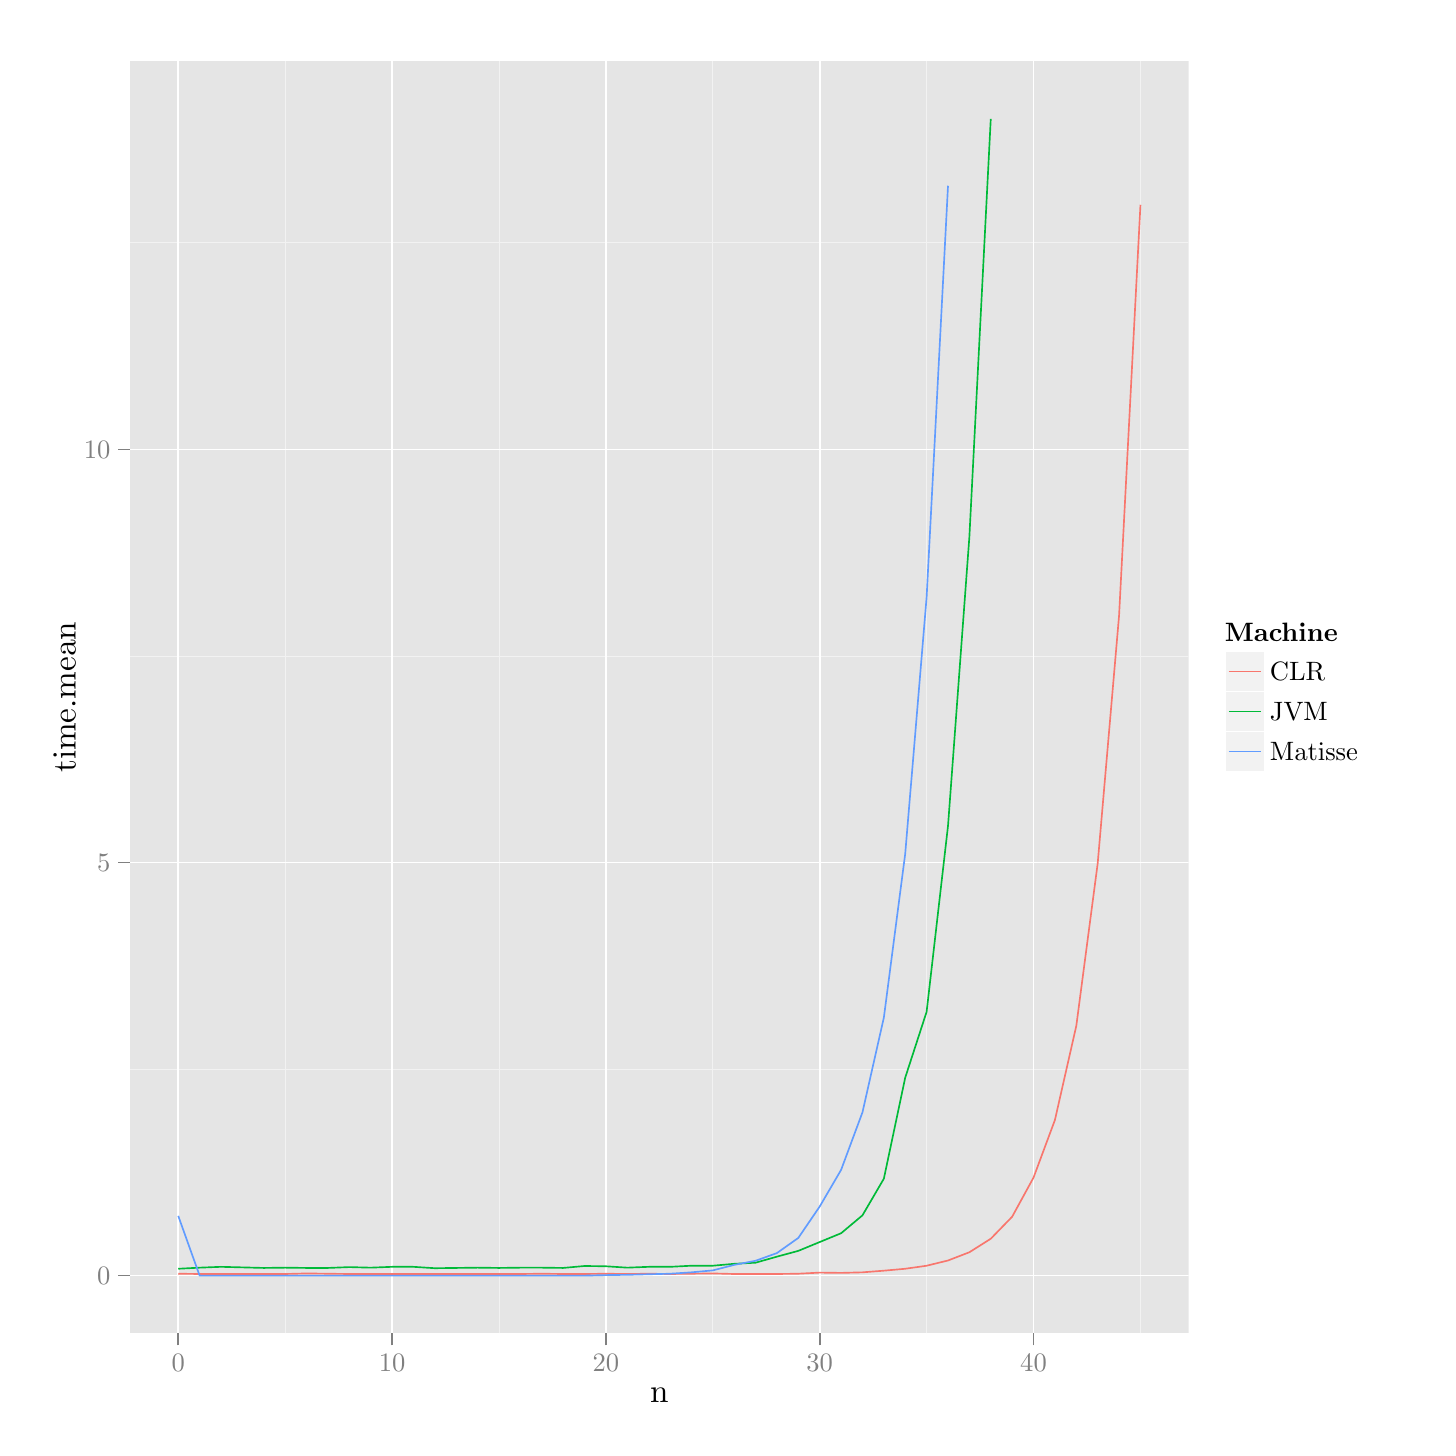
\begin{tikzpicture}[x=1pt,y=1pt]
\definecolor{fillColor}{RGB}{255,255,255}
\path[use as bounding box,fill=fillColor,fill opacity=0.00] (0,0) rectangle (505.89,505.89);
\begin{scope}
\path[clip] (  0.00,  0.00) rectangle (505.89,505.89);
\definecolor{drawColor}{RGB}{255,255,255}
\definecolor{fillColor}{RGB}{255,255,255}

\path[draw=drawColor,line width= 0.6pt,line join=round,line cap=round,fill=fillColor] (  0.00,  0.00) rectangle (505.89,505.89);
\end{scope}
\begin{scope}
\path[clip] ( 37.02, 34.03) rectangle (419.48,493.85);
\definecolor{fillColor}{gray}{0.90}

\path[fill=fillColor] ( 37.02, 34.03) rectangle (419.48,493.85);
\definecolor{drawColor}{gray}{0.95}

\path[draw=drawColor,line width= 0.3pt,line join=round] ( 37.02,129.58) --
	(419.48,129.58);

\path[draw=drawColor,line width= 0.3pt,line join=round] ( 37.02,278.87) --
	(419.48,278.87);

\path[draw=drawColor,line width= 0.3pt,line join=round] ( 37.02,428.16) --
	(419.48,428.16);

\path[draw=drawColor,line width= 0.3pt,line join=round] ( 93.04, 34.03) --
	( 93.04,493.85);

\path[draw=drawColor,line width= 0.3pt,line join=round] (170.30, 34.03) --
	(170.30,493.85);

\path[draw=drawColor,line width= 0.3pt,line join=round] (247.57, 34.03) --
	(247.57,493.85);

\path[draw=drawColor,line width= 0.3pt,line join=round] (324.83, 34.03) --
	(324.83,493.85);

\path[draw=drawColor,line width= 0.3pt,line join=round] (402.10, 34.03) --
	(402.10,493.85);
\definecolor{drawColor}{RGB}{255,255,255}

\path[draw=drawColor,line width= 0.6pt,line join=round] ( 37.02, 54.94) --
	(419.48, 54.94);

\path[draw=drawColor,line width= 0.6pt,line join=round] ( 37.02,204.22) --
	(419.48,204.22);

\path[draw=drawColor,line width= 0.6pt,line join=round] ( 37.02,353.51) --
	(419.48,353.51);

\path[draw=drawColor,line width= 0.6pt,line join=round] ( 54.41, 34.03) --
	( 54.41,493.85);

\path[draw=drawColor,line width= 0.6pt,line join=round] (131.67, 34.03) --
	(131.67,493.85);

\path[draw=drawColor,line width= 0.6pt,line join=round] (208.93, 34.03) --
	(208.93,493.85);

\path[draw=drawColor,line width= 0.6pt,line join=round] (286.20, 34.03) --
	(286.20,493.85);

\path[draw=drawColor,line width= 0.6pt,line join=round] (363.46, 34.03) --
	(363.46,493.85);
\definecolor{drawColor}{RGB}{248,118,109}

\path[draw=drawColor,line width= 0.6pt,line join=round] ( 54.41, 55.63) --
	( 62.13, 55.53) --
	( 69.86, 55.53) --
	( 77.58, 55.53) --
	( 85.31, 55.53) --
	( 93.04, 55.53) --
	(100.76, 55.73) --
	(108.49, 55.63) --
	(116.22, 55.53) --
	(123.94, 55.53) --
	(131.67, 55.53) --
	(139.40, 55.53) --
	(147.12, 55.53) --
	(154.85, 55.53) --
	(162.58, 55.53) --
	(170.30, 55.53) --
	(178.03, 55.53) --
	(185.75, 55.63) --
	(193.48, 55.53) --
	(201.21, 55.53) --
	(208.93, 55.63) --
	(216.66, 55.53) --
	(224.39, 55.63) --
	(232.11, 55.53) --
	(239.84, 55.63) --
	(247.57, 55.73) --
	(255.29, 55.53) --
	(263.02, 55.53) --
	(270.75, 55.53) --
	(278.47, 55.63) --
	(286.20, 56.03) --
	(293.93, 55.93) --
	(301.65, 56.13) --
	(309.38, 56.73) --
	(317.10, 57.42) --
	(324.83, 58.52) --
	(332.56, 60.41) --
	(340.28, 63.39) --
	(348.01, 68.27) --
	(355.74, 76.23) --
	(363.46, 90.37) --
	(371.19,111.17) --
	(378.92,145.21) --
	(386.64,203.83) --
	(394.37,293.40) --
	(402.10,441.89);
\definecolor{drawColor}{RGB}{0,186,56}

\path[draw=drawColor,line width= 0.6pt,line join=round] ( 54.41, 57.42) --
	( 62.13, 57.82) --
	( 69.86, 58.12) --
	( 77.58, 57.92) --
	( 85.31, 57.72) --
	( 93.04, 57.82) --
	(100.76, 57.72) --
	(108.49, 57.72) --
	(116.22, 58.02) --
	(123.94, 57.82) --
	(131.67, 58.12) --
	(139.40, 58.12) --
	(147.12, 57.62) --
	(154.85, 57.72) --
	(162.58, 57.82) --
	(170.30, 57.72) --
	(178.03, 57.82) --
	(185.75, 57.82) --
	(193.48, 57.72) --
	(201.21, 58.42) --
	(208.93, 58.32) --
	(216.66, 57.82) --
	(224.39, 58.12) --
	(232.11, 58.12) --
	(239.84, 58.52) --
	(247.57, 58.52) --
	(255.29, 59.21) --
	(263.02, 59.61) --
	(270.75, 61.80) --
	(278.47, 63.89) --
	(286.20, 67.08) --
	(293.93, 70.26) --
	(301.65, 76.73) --
	(309.38, 89.97) --
	(317.10,126.49) --
	(324.83,150.28) --
	(332.56,217.46) --
	(340.28,321.86) --
	(348.01,472.94);
\definecolor{drawColor}{RGB}{97,156,255}

\path[draw=drawColor,line width= 0.6pt,line join=round] ( 54.41, 76.53) --
	( 62.13, 54.94) --
	( 69.86, 54.94) --
	( 77.58, 54.94) --
	( 85.31, 54.94) --
	( 93.04, 54.94) --
	(100.76, 54.94) --
	(108.49, 54.94) --
	(116.22, 54.94) --
	(123.94, 54.94) --
	(131.67, 54.94) --
	(139.40, 54.94) --
	(147.12, 54.94) --
	(154.85, 54.94) --
	(162.58, 54.94) --
	(170.30, 54.94) --
	(178.03, 54.94) --
	(185.75, 54.94) --
	(193.48, 54.94) --
	(201.21, 54.94) --
	(208.93, 55.13) --
	(216.66, 55.23) --
	(224.39, 55.43) --
	(232.11, 55.63) --
	(239.84, 56.13) --
	(247.57, 56.83) --
	(255.29, 58.82) --
	(263.02, 60.31) --
	(270.75, 63.10) --
	(278.47, 68.57) --
	(286.20, 79.92) --
	(293.93, 93.15) --
	(301.65,113.95) --
	(309.38,148.19) --
	(317.10,207.41) --
	(324.83,300.07) --
	(332.56,448.76);
\end{scope}
\begin{scope}
\path[clip] (  0.00,  0.00) rectangle (505.89,505.89);
\definecolor{drawColor}{gray}{0.50}

\node[text=drawColor,anchor=base east,inner sep=0pt, outer sep=0pt, scale=  0.96] at ( 29.91, 51.63) {0};

\node[text=drawColor,anchor=base east,inner sep=0pt, outer sep=0pt, scale=  0.96] at ( 29.91,200.92) {5};

\node[text=drawColor,anchor=base east,inner sep=0pt, outer sep=0pt, scale=  0.96] at ( 29.91,350.21) {10};
\end{scope}
\begin{scope}
\path[clip] (  0.00,  0.00) rectangle (505.89,505.89);
\definecolor{drawColor}{gray}{0.50}

\path[draw=drawColor,line width= 0.6pt,line join=round] ( 32.75, 54.94) --
	( 37.02, 54.94);

\path[draw=drawColor,line width= 0.6pt,line join=round] ( 32.75,204.22) --
	( 37.02,204.22);

\path[draw=drawColor,line width= 0.6pt,line join=round] ( 32.75,353.51) --
	( 37.02,353.51);
\end{scope}
\begin{scope}
\path[clip] (  0.00,  0.00) rectangle (505.89,505.89);
\definecolor{drawColor}{gray}{0.50}

\path[draw=drawColor,line width= 0.6pt,line join=round] ( 54.41, 29.77) --
	( 54.41, 34.03);

\path[draw=drawColor,line width= 0.6pt,line join=round] (131.67, 29.77) --
	(131.67, 34.03);

\path[draw=drawColor,line width= 0.6pt,line join=round] (208.93, 29.77) --
	(208.93, 34.03);

\path[draw=drawColor,line width= 0.6pt,line join=round] (286.20, 29.77) --
	(286.20, 34.03);

\path[draw=drawColor,line width= 0.6pt,line join=round] (363.46, 29.77) --
	(363.46, 34.03);
\end{scope}
\begin{scope}
\path[clip] (  0.00,  0.00) rectangle (505.89,505.89);
\definecolor{drawColor}{gray}{0.50}

\node[text=drawColor,anchor=base,inner sep=0pt, outer sep=0pt, scale=  0.96] at ( 54.41, 20.31) {0};

\node[text=drawColor,anchor=base,inner sep=0pt, outer sep=0pt, scale=  0.96] at (131.67, 20.31) {10};

\node[text=drawColor,anchor=base,inner sep=0pt, outer sep=0pt, scale=  0.96] at (208.93, 20.31) {20};

\node[text=drawColor,anchor=base,inner sep=0pt, outer sep=0pt, scale=  0.96] at (286.20, 20.31) {30};

\node[text=drawColor,anchor=base,inner sep=0pt, outer sep=0pt, scale=  0.96] at (363.46, 20.31) {40};
\end{scope}
\begin{scope}
\path[clip] (  0.00,  0.00) rectangle (505.89,505.89);
\definecolor{drawColor}{RGB}{0,0,0}

\node[text=drawColor,anchor=base,inner sep=0pt, outer sep=0pt, scale=  1.20] at (228.25,  9.03) {n};
\end{scope}
\begin{scope}
\path[clip] (  0.00,  0.00) rectangle (505.89,505.89);
\definecolor{drawColor}{RGB}{0,0,0}

\node[text=drawColor,rotate= 90.00,anchor=base,inner sep=0pt, outer sep=0pt, scale=  1.20] at ( 17.30,263.94) {time.mean};
\end{scope}
\begin{scope}
\path[clip] (  0.00,  0.00) rectangle (505.89,505.89);
\definecolor{fillColor}{RGB}{255,255,255}

\path[fill=fillColor] (428.35,232.87) rectangle (484.98,295.01);
\end{scope}
\begin{scope}
\path[clip] (  0.00,  0.00) rectangle (505.89,505.89);
\definecolor{drawColor}{RGB}{0,0,0}

\node[text=drawColor,anchor=base west,inner sep=0pt, outer sep=0pt, scale=  0.96] at (432.62,284.11) {\bfseries Machine};
\end{scope}
\begin{scope}
\path[clip] (  0.00,  0.00) rectangle (505.89,505.89);
\definecolor{drawColor}{RGB}{255,255,255}
\definecolor{fillColor}{gray}{0.95}

\path[draw=drawColor,line width= 0.6pt,line join=round,line cap=round,fill=fillColor] (432.62,266.05) rectangle (447.07,280.50);
\end{scope}
\begin{scope}
\path[clip] (  0.00,  0.00) rectangle (505.89,505.89);
\definecolor{drawColor}{RGB}{248,118,109}

\path[draw=drawColor,line width= 0.6pt,line join=round] (434.06,273.27) -- (445.62,273.27);
\end{scope}
\begin{scope}
\path[clip] (  0.00,  0.00) rectangle (505.89,505.89);
\definecolor{drawColor}{RGB}{255,255,255}
\definecolor{fillColor}{gray}{0.95}

\path[draw=drawColor,line width= 0.6pt,line join=round,line cap=round,fill=fillColor] (432.62,251.59) rectangle (447.07,266.05);
\end{scope}
\begin{scope}
\path[clip] (  0.00,  0.00) rectangle (505.89,505.89);
\definecolor{drawColor}{RGB}{0,186,56}

\path[draw=drawColor,line width= 0.6pt,line join=round] (434.06,258.82) -- (445.62,258.82);
\end{scope}
\begin{scope}
\path[clip] (  0.00,  0.00) rectangle (505.89,505.89);
\definecolor{drawColor}{RGB}{255,255,255}
\definecolor{fillColor}{gray}{0.95}

\path[draw=drawColor,line width= 0.6pt,line join=round,line cap=round,fill=fillColor] (432.62,237.14) rectangle (447.07,251.59);
\end{scope}
\begin{scope}
\path[clip] (  0.00,  0.00) rectangle (505.89,505.89);
\definecolor{drawColor}{RGB}{97,156,255}

\path[draw=drawColor,line width= 0.6pt,line join=round] (434.06,244.37) -- (445.62,244.37);
\end{scope}
\begin{scope}
\path[clip] (  0.00,  0.00) rectangle (505.89,505.89);
\definecolor{drawColor}{RGB}{0,0,0}

\node[text=drawColor,anchor=base west,inner sep=0pt, outer sep=0pt, scale=  0.96] at (448.88,269.97) {CLR};
\end{scope}
\begin{scope}
\path[clip] (  0.00,  0.00) rectangle (505.89,505.89);
\definecolor{drawColor}{RGB}{0,0,0}

\node[text=drawColor,anchor=base west,inner sep=0pt, outer sep=0pt, scale=  0.96] at (448.88,255.51) {JVM};
\end{scope}
\begin{scope}
\path[clip] (  0.00,  0.00) rectangle (505.89,505.89);
\definecolor{drawColor}{RGB}{0,0,0}

\node[text=drawColor,anchor=base west,inner sep=0pt, outer sep=0pt, scale=  0.96] at (448.88,241.06) {Matisse};
\end{scope}
\end{tikzpicture}
}
      \captionof{figure}{Fibonacci}
    \end{minipage}%
    \begin{minipage}{.5\textwidth}
      \centering
          \scalebox{0.36}[0.3]{% Created by tikzDevice version 0.8.1 on 2015-06-28 20:20:30
% !TEX encoding = UTF-8 Unicode
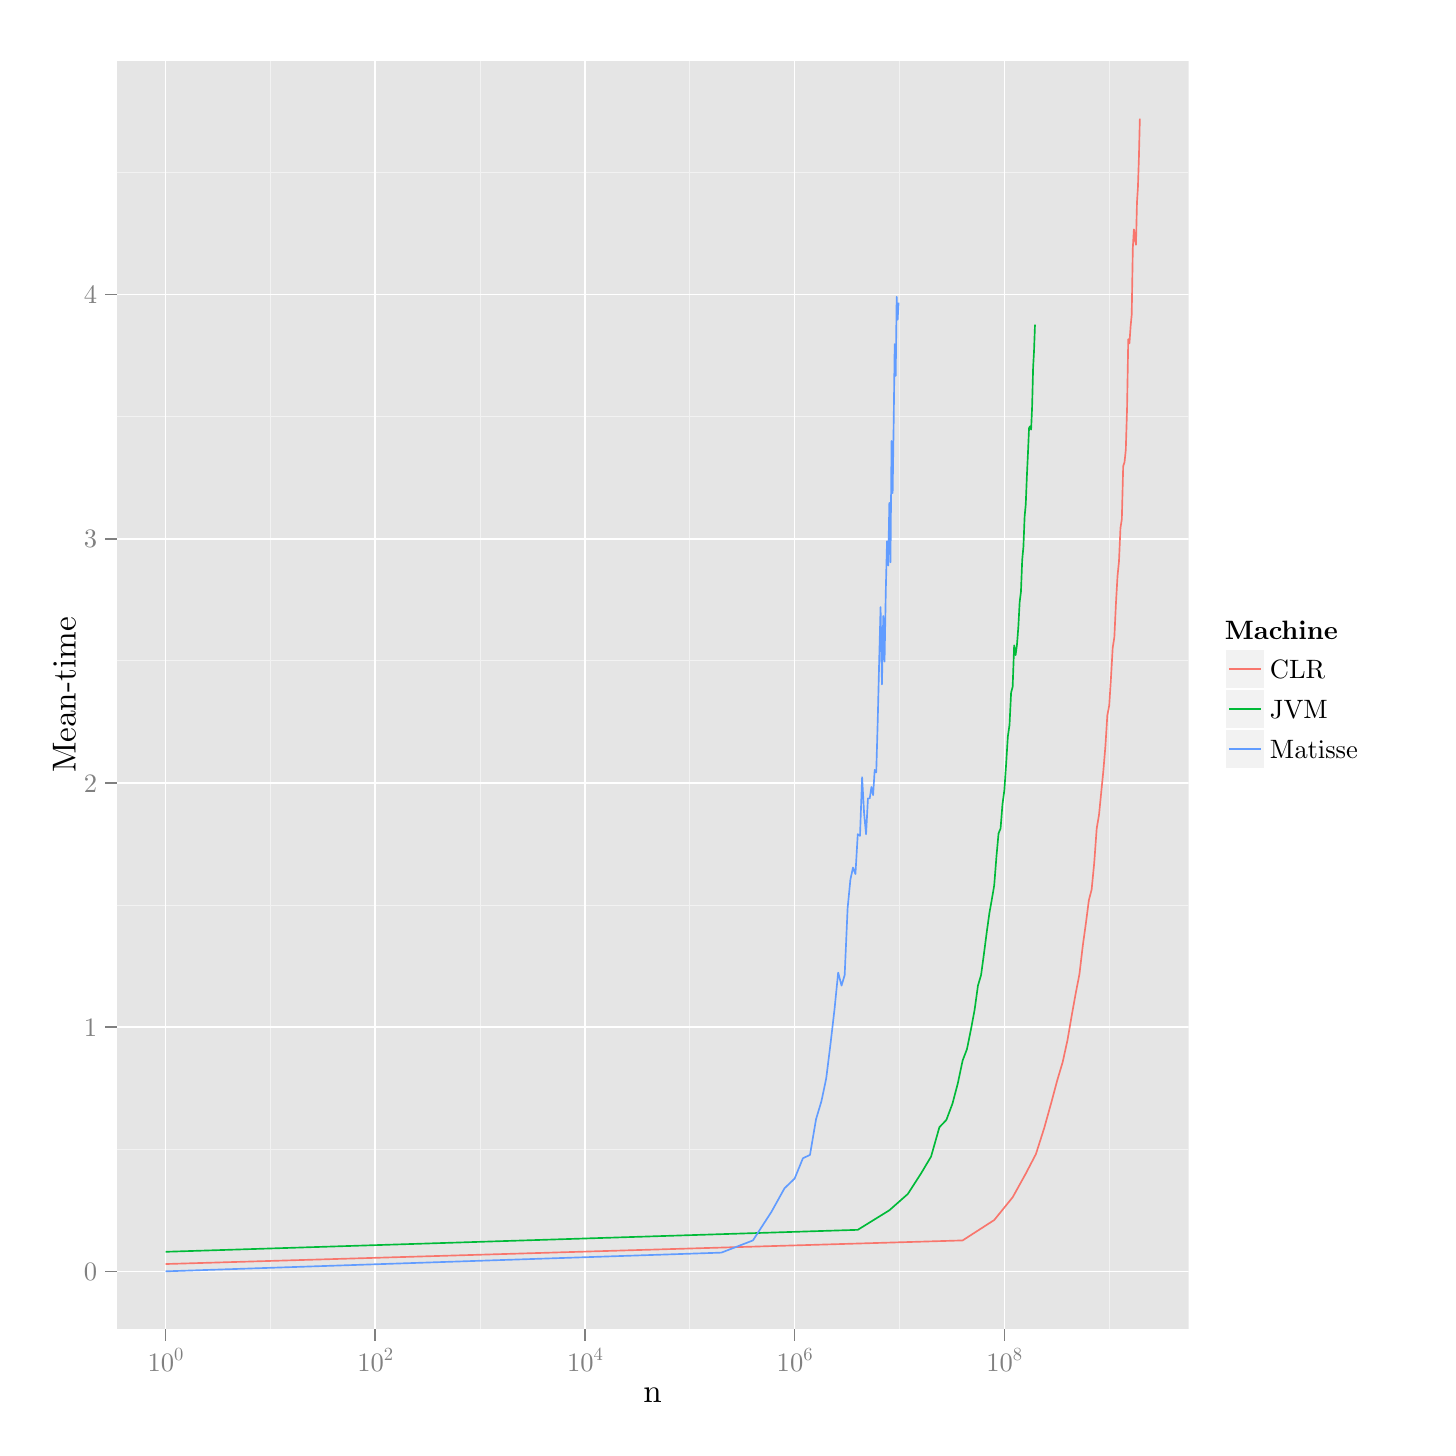
\begin{tikzpicture}[x=1pt,y=1pt]
\definecolor{fillColor}{RGB}{255,255,255}
\path[use as bounding box,fill=fillColor,fill opacity=0.00] (0,0) rectangle (505.89,505.89);
\begin{scope}
\path[clip] (  0.00,  0.00) rectangle (505.89,505.89);
\definecolor{drawColor}{RGB}{255,255,255}
\definecolor{fillColor}{RGB}{255,255,255}

\path[draw=drawColor,line width= 0.6pt,line join=round,line cap=round,fill=fillColor] (  0.00,  0.00) rectangle (505.89,505.89);
\end{scope}
\begin{scope}
\path[clip] ( 32.22, 35.66) rectangle (419.48,493.85);
\definecolor{fillColor}{gray}{0.90}

\path[fill=fillColor] ( 32.22, 35.66) rectangle (419.48,493.85);
\definecolor{drawColor}{gray}{0.95}

\path[draw=drawColor,line width= 0.3pt,line join=round] ( 32.22,100.61) --
	(419.48,100.61);

\path[draw=drawColor,line width= 0.3pt,line join=round] ( 32.22,188.86) --
	(419.48,188.86);

\path[draw=drawColor,line width= 0.3pt,line join=round] ( 32.22,277.11) --
	(419.48,277.11);

\path[draw=drawColor,line width= 0.3pt,line join=round] ( 32.22,365.36) --
	(419.48,365.36);

\path[draw=drawColor,line width= 0.3pt,line join=round] ( 32.22,453.60) --
	(419.48,453.60);

\path[draw=drawColor,line width= 0.3pt,line join=round] ( 87.71, 35.66) --
	( 87.71,493.85);

\path[draw=drawColor,line width= 0.3pt,line join=round] (163.48, 35.66) --
	(163.48,493.85);

\path[draw=drawColor,line width= 0.3pt,line join=round] (239.26, 35.66) --
	(239.26,493.85);

\path[draw=drawColor,line width= 0.3pt,line join=round] (315.03, 35.66) --
	(315.03,493.85);

\path[draw=drawColor,line width= 0.3pt,line join=round] (390.81, 35.66) --
	(390.81,493.85);
\definecolor{drawColor}{RGB}{255,255,255}

\path[draw=drawColor,line width= 0.6pt,line join=round] ( 32.22, 56.49) --
	(419.48, 56.49);

\path[draw=drawColor,line width= 0.6pt,line join=round] ( 32.22,144.73) --
	(419.48,144.73);

\path[draw=drawColor,line width= 0.6pt,line join=round] ( 32.22,232.98) --
	(419.48,232.98);

\path[draw=drawColor,line width= 0.6pt,line join=round] ( 32.22,321.23) --
	(419.48,321.23);

\path[draw=drawColor,line width= 0.6pt,line join=round] ( 32.22,409.48) --
	(419.48,409.48);

\path[draw=drawColor,line width= 0.6pt,line join=round] ( 49.82, 35.66) --
	( 49.82,493.85);

\path[draw=drawColor,line width= 0.6pt,line join=round] (125.60, 35.66) --
	(125.60,493.85);

\path[draw=drawColor,line width= 0.6pt,line join=round] (201.37, 35.66) --
	(201.37,493.85);

\path[draw=drawColor,line width= 0.6pt,line join=round] (277.14, 35.66) --
	(277.14,493.85);

\path[draw=drawColor,line width= 0.6pt,line join=round] (352.92, 35.66) --
	(352.92,493.85);
\definecolor{drawColor}{RGB}{248,118,109}

\path[draw=drawColor,line width= 0.6pt,line join=round] ( 49.82, 59.13) --
	(337.84, 67.66) --
	(349.25, 75.02) --
	(355.92, 83.25) --
	(360.65, 91.79) --
	(364.32, 98.85) --
	(367.32,108.26) --
	(369.86,117.38) --
	(372.06,125.61) --
	(373.99,132.09) --
	(375.73,140.03) --
	(377.30,149.15) --
	(378.73,157.09) --
	(380.05,163.85) --
	(381.26,174.15) --
	(382.40,182.39) --
	(383.46,190.62) --
	(384.46,194.45) --
	(385.40,204.16) --
	(386.29,216.51) --
	(387.13,221.51) --
	(387.94,229.75) --
	(388.70,237.40) --
	(389.43,246.22) --
	(390.13,257.40) --
	(390.81,260.93) --
	(391.45,270.93) --
	(392.07,281.81) --
	(392.67,285.64) --
	(393.25,297.99) --
	(393.81,307.70) --
	(394.34,312.99) --
	(394.87,325.06) --
	(395.37,328.29) --
	(395.86,347.41) --
	(396.34,348.88) --
	(396.80,353.29) --
	(397.26,368.30) --
	(397.69,393.30) --
	(398.12,391.83) --
	(398.54,398.01) --
	(398.94,402.13) --
	(399.34,426.25) --
	(399.73,433.01) --
	(400.11,429.48) --
	(400.48,427.42) --
	(400.84,442.72) --
	(401.19,448.31) --
	(401.54,458.90) --
	(401.88,473.02);
\definecolor{drawColor}{RGB}{0,186,56}

\path[draw=drawColor,line width= 0.6pt,line join=round] ( 49.82, 63.55) --
	(299.95, 71.49) --
	(311.36, 78.55) --
	(318.03, 84.43) --
	(322.77, 91.79) --
	(326.44, 97.96) --
	(329.44,108.55) --
	(331.97,111.20) --
	(334.17,117.08) --
	(336.11,124.44) --
	(337.84,132.67) --
	(339.41,136.79) --
	(340.84,143.85) --
	(342.16,150.91) --
	(343.38,159.74) --
	(344.51,163.56) --
	(345.58,171.50) --
	(346.57,179.15) --
	(347.51,185.92) --
	(348.40,190.92) --
	(349.25,195.92) --
	(350.05,206.21) --
	(350.82,214.74) --
	(351.55,216.51) --
	(352.25,225.33) --
	(352.92,230.34) --
	(353.56,239.75) --
	(354.18,249.75) --
	(354.78,253.87) --
	(355.36,265.63) --
	(355.92,267.69) --
	(356.46,282.70) --
	(356.98,279.17) --
	(357.49,282.99) --
	(357.98,289.46) --
	(358.45,298.29) --
	(358.92,302.11) --
	(359.37,313.58) --
	(359.81,318.29) --
	(360.24,329.17) --
	(360.65,333.59) --
	(361.06,343.88) --
	(361.45,352.12) --
	(361.84,361.24) --
	(362.22,361.83) --
	(362.59,360.65) --
	(362.95,368.89) --
	(363.31,383.01) --
	(363.65,389.18) --
	(363.99,398.60);
\definecolor{drawColor}{RGB}{97,156,255}

\path[draw=drawColor,line width= 0.6pt,line join=round] ( 49.82, 56.49) --
	(250.66, 63.25) --
	(262.07, 67.66) --
	(268.74, 77.96) --
	(273.47, 86.49) --
	(277.14, 90.02) --
	(280.14, 97.37) --
	(282.68, 98.55) --
	(284.88,111.49) --
	(286.82,117.97) --
	(288.55,126.20) --
	(290.12,138.85) --
	(291.55,151.21) --
	(292.87,164.44) --
	(294.09,159.74) --
	(295.22,163.56) --
	(296.28,187.68) --
	(297.28,197.98) --
	(298.22,202.39) --
	(299.11,200.04) --
	(299.95,214.45) --
	(300.76,213.86) --
	(301.52,235.04) --
	(302.25,221.80) --
	(302.95,214.45) --
	(303.63,227.39) --
	(304.27,227.39) --
	(304.89,231.51) --
	(305.49,228.57) --
	(306.07,237.69) --
	(306.63,236.81) --
	(307.17,255.63) --
	(307.69,277.11) --
	(308.19,296.52) --
	(308.69,268.58) --
	(309.16,293.29) --
	(309.63,276.81) --
	(310.08,302.40) --
	(310.52,320.35) --
	(310.94,311.52) --
	(311.36,334.17) --
	(311.77,312.70) --
	(312.16,356.53) --
	(312.55,337.70) --
	(312.93,363.30) --
	(313.30,391.54) --
	(313.66,380.06) --
	(314.01,408.60) --
	(314.36,400.36) --
	(314.70,406.54);
\end{scope}
\begin{scope}
\path[clip] (  0.00,  0.00) rectangle (505.89,505.89);
\definecolor{drawColor}{gray}{0.50}

\node[text=drawColor,anchor=base east,inner sep=0pt, outer sep=0pt, scale=  0.96] at ( 25.11, 53.18) {0};

\node[text=drawColor,anchor=base east,inner sep=0pt, outer sep=0pt, scale=  0.96] at ( 25.11,141.43) {1};

\node[text=drawColor,anchor=base east,inner sep=0pt, outer sep=0pt, scale=  0.96] at ( 25.11,229.68) {2};

\node[text=drawColor,anchor=base east,inner sep=0pt, outer sep=0pt, scale=  0.96] at ( 25.11,317.93) {3};

\node[text=drawColor,anchor=base east,inner sep=0pt, outer sep=0pt, scale=  0.96] at ( 25.11,406.17) {4};
\end{scope}
\begin{scope}
\path[clip] (  0.00,  0.00) rectangle (505.89,505.89);
\definecolor{drawColor}{gray}{0.50}

\path[draw=drawColor,line width= 0.6pt,line join=round] ( 27.95, 56.49) --
	( 32.22, 56.49);

\path[draw=drawColor,line width= 0.6pt,line join=round] ( 27.95,144.73) --
	( 32.22,144.73);

\path[draw=drawColor,line width= 0.6pt,line join=round] ( 27.95,232.98) --
	( 32.22,232.98);

\path[draw=drawColor,line width= 0.6pt,line join=round] ( 27.95,321.23) --
	( 32.22,321.23);

\path[draw=drawColor,line width= 0.6pt,line join=round] ( 27.95,409.48) --
	( 32.22,409.48);
\end{scope}
\begin{scope}
\path[clip] (  0.00,  0.00) rectangle (505.89,505.89);
\definecolor{drawColor}{gray}{0.50}

\path[draw=drawColor,line width= 0.6pt,line join=round] ( 49.82, 31.39) --
	( 49.82, 35.66);

\path[draw=drawColor,line width= 0.6pt,line join=round] (125.60, 31.39) --
	(125.60, 35.66);

\path[draw=drawColor,line width= 0.6pt,line join=round] (201.37, 31.39) --
	(201.37, 35.66);

\path[draw=drawColor,line width= 0.6pt,line join=round] (277.14, 31.39) --
	(277.14, 35.66);

\path[draw=drawColor,line width= 0.6pt,line join=round] (352.92, 31.39) --
	(352.92, 35.66);
\end{scope}
\begin{scope}
\path[clip] (  0.00,  0.00) rectangle (505.89,505.89);
\definecolor{drawColor}{gray}{0.50}

\node[text=drawColor,anchor=base west,inner sep=0pt, outer sep=0pt, scale=  0.96] at ( 43.35, 20.31) {10};

\node[text=drawColor,anchor=base west,inner sep=0pt, outer sep=0pt, scale=  0.67] at ( 52.94, 24.24) {0};

\node[text=drawColor,anchor=base west,inner sep=0pt, outer sep=0pt, scale=  0.96] at (119.12, 20.31) {10};

\node[text=drawColor,anchor=base west,inner sep=0pt, outer sep=0pt, scale=  0.67] at (128.72, 24.24) {2};

\node[text=drawColor,anchor=base west,inner sep=0pt, outer sep=0pt, scale=  0.96] at (194.89, 20.31) {10};

\node[text=drawColor,anchor=base west,inner sep=0pt, outer sep=0pt, scale=  0.67] at (204.49, 24.24) {4};

\node[text=drawColor,anchor=base west,inner sep=0pt, outer sep=0pt, scale=  0.96] at (270.67, 20.31) {10};

\node[text=drawColor,anchor=base west,inner sep=0pt, outer sep=0pt, scale=  0.67] at (280.26, 24.24) {6};

\node[text=drawColor,anchor=base west,inner sep=0pt, outer sep=0pt, scale=  0.96] at (346.44, 20.31) {10};

\node[text=drawColor,anchor=base west,inner sep=0pt, outer sep=0pt, scale=  0.67] at (356.04, 24.24) {8};
\end{scope}
\begin{scope}
\path[clip] (  0.00,  0.00) rectangle (505.89,505.89);
\definecolor{drawColor}{RGB}{0,0,0}

\node[text=drawColor,anchor=base,inner sep=0pt, outer sep=0pt, scale=  1.20] at (225.85,  9.03) {n};
\end{scope}
\begin{scope}
\path[clip] (  0.00,  0.00) rectangle (505.89,505.89);
\definecolor{drawColor}{RGB}{0,0,0}

\node[text=drawColor,rotate= 90.00,anchor=base,inner sep=0pt, outer sep=0pt, scale=  1.20] at ( 17.30,264.75) {Mean-time};
\end{scope}
\begin{scope}
\path[clip] (  0.00,  0.00) rectangle (505.89,505.89);
\definecolor{fillColor}{RGB}{255,255,255}

\path[fill=fillColor] (428.35,233.68) rectangle (484.98,295.82);
\end{scope}
\begin{scope}
\path[clip] (  0.00,  0.00) rectangle (505.89,505.89);
\definecolor{drawColor}{RGB}{0,0,0}

\node[text=drawColor,anchor=base west,inner sep=0pt, outer sep=0pt, scale=  0.96] at (432.62,284.93) {\bfseries Machine};
\end{scope}
\begin{scope}
\path[clip] (  0.00,  0.00) rectangle (505.89,505.89);
\definecolor{drawColor}{RGB}{255,255,255}
\definecolor{fillColor}{gray}{0.95}

\path[draw=drawColor,line width= 0.6pt,line join=round,line cap=round,fill=fillColor] (432.62,266.86) rectangle (447.07,281.31);
\end{scope}
\begin{scope}
\path[clip] (  0.00,  0.00) rectangle (505.89,505.89);
\definecolor{drawColor}{RGB}{248,118,109}

\path[draw=drawColor,line width= 0.6pt,line join=round] (434.06,274.09) -- (445.62,274.09);
\end{scope}
\begin{scope}
\path[clip] (  0.00,  0.00) rectangle (505.89,505.89);
\definecolor{drawColor}{RGB}{255,255,255}
\definecolor{fillColor}{gray}{0.95}

\path[draw=drawColor,line width= 0.6pt,line join=round,line cap=round,fill=fillColor] (432.62,252.41) rectangle (447.07,266.86);
\end{scope}
\begin{scope}
\path[clip] (  0.00,  0.00) rectangle (505.89,505.89);
\definecolor{drawColor}{RGB}{0,186,56}

\path[draw=drawColor,line width= 0.6pt,line join=round] (434.06,259.63) -- (445.62,259.63);
\end{scope}
\begin{scope}
\path[clip] (  0.00,  0.00) rectangle (505.89,505.89);
\definecolor{drawColor}{RGB}{255,255,255}
\definecolor{fillColor}{gray}{0.95}

\path[draw=drawColor,line width= 0.6pt,line join=round,line cap=round,fill=fillColor] (432.62,237.95) rectangle (447.07,252.41);
\end{scope}
\begin{scope}
\path[clip] (  0.00,  0.00) rectangle (505.89,505.89);
\definecolor{drawColor}{RGB}{97,156,255}

\path[draw=drawColor,line width= 0.6pt,line join=round] (434.06,245.18) -- (445.62,245.18);
\end{scope}
\begin{scope}
\path[clip] (  0.00,  0.00) rectangle (505.89,505.89);
\definecolor{drawColor}{RGB}{0,0,0}

\node[text=drawColor,anchor=base west,inner sep=0pt, outer sep=0pt, scale=  0.96] at (448.88,270.78) {CLR};
\end{scope}
\begin{scope}
\path[clip] (  0.00,  0.00) rectangle (505.89,505.89);
\definecolor{drawColor}{RGB}{0,0,0}

\node[text=drawColor,anchor=base west,inner sep=0pt, outer sep=0pt, scale=  0.96] at (448.88,256.33) {JVM};
\end{scope}
\begin{scope}
\path[clip] (  0.00,  0.00) rectangle (505.89,505.89);
\definecolor{drawColor}{RGB}{0,0,0}

\node[text=drawColor,anchor=base west,inner sep=0pt, outer sep=0pt, scale=  0.96] at (448.88,241.87) {Matisse};
\end{scope}
\end{tikzpicture}
}
      \captionof{figure}{Heap Workout}
    \end{minipage}
  \end{figure}
\end{frame}

\begin{frame}
  \frametitle{Performance Evaluation}
  \framesubtitle{Memory Footprint}

  \begin{figure}[H]
    \centering
    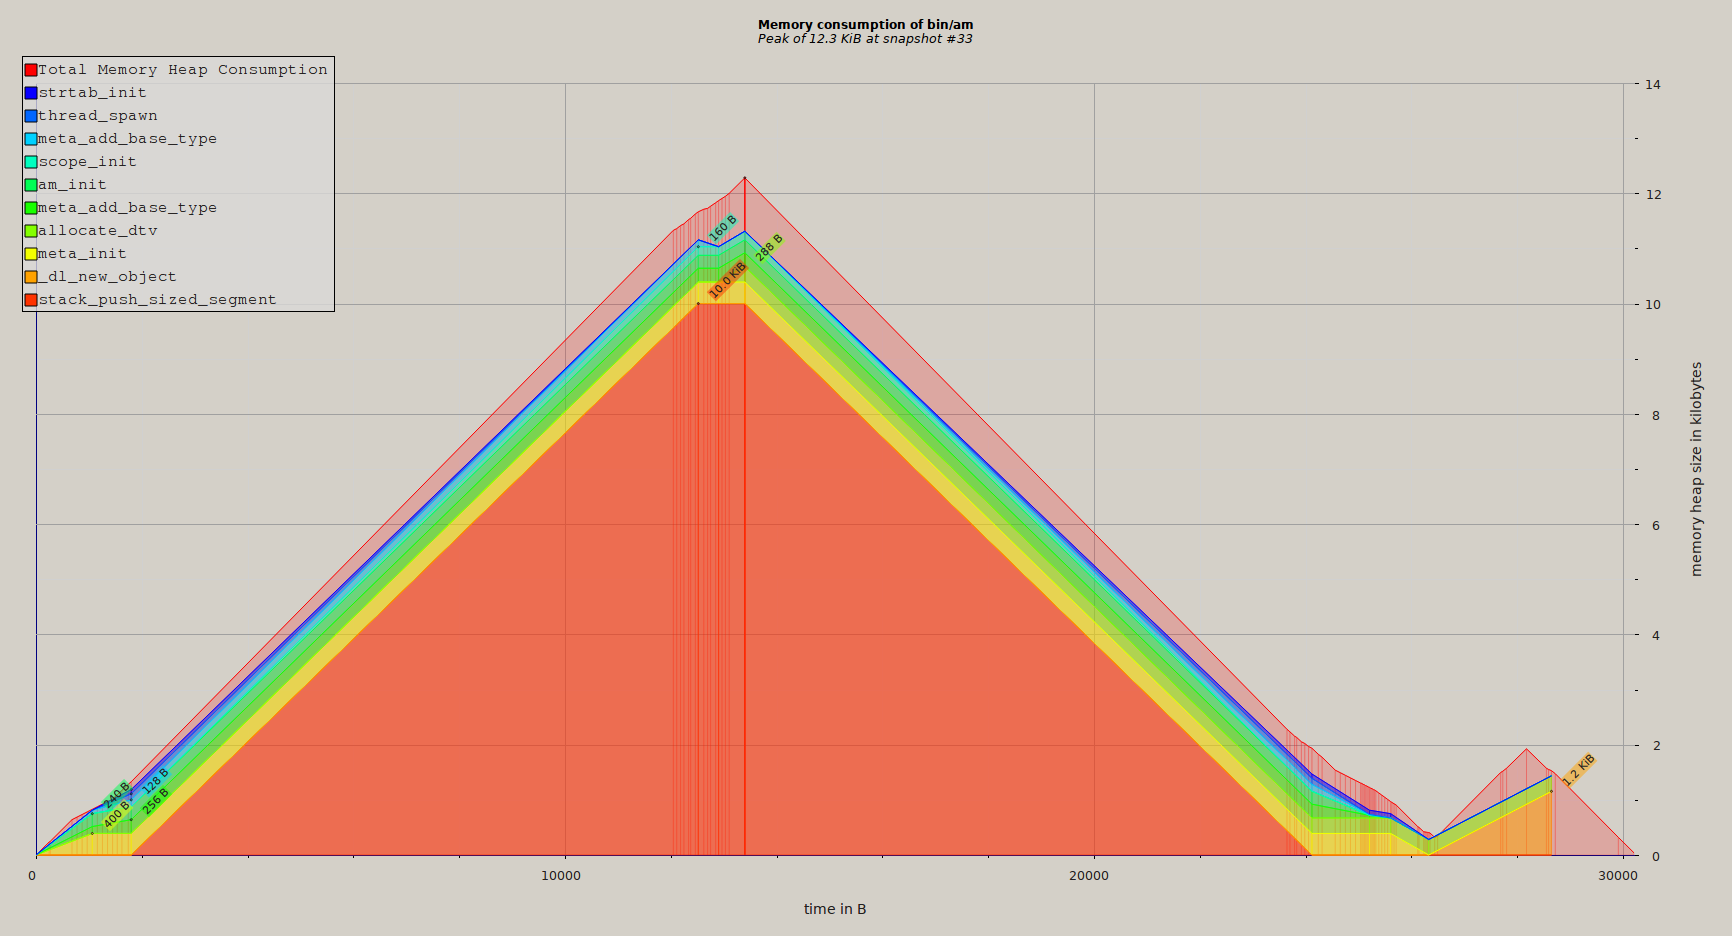
\includegraphics[scale=0.23]{../figures/fig-mem}
    \caption{Fibonacci}
  \end{figure}
\end{frame}

\begin{frame}
  \frametitle{Conclusions}

  \begin{itemize}
  \item Did we succeed?
    \n{A good proof-of-concept, basics work, performance is bad (expected)}
  \item What we learned
    \n{AM internals, primitives needed for language impl., C design and architecture}
  \item Future of Matisse
    \n{More implementation}
  \end{itemize}
\end{frame}

\end{document}
%%% Local Variables:
%%% mode: latex
%%% TeX-master: t
%%% End:
